% 日本語技術報告書原稿（LuaLaTeXでコンパイル）
\documentclass[11pt,a4paper]{ltjsarticle}

\usepackage[margin=25mm]{geometry}
\usepackage{amsmath}
\usepackage{array}
\usepackage{booktabs}
\usepackage{graphicx}
\usepackage{hyperref}
\usepackage{multirow}
\usepackage{tabularx}
\hypersetup{hidelinks}
\graphicspath{{figure/}}

\title{発話が表す意図と意味の近い意図との違いを説明する文章を用いたSpeechLLMの意図分類性能向上}
\author{}
\date{}

\begin{document}

\maketitle

\begin{abstract}
近年、音声大規模言語モデル（SpeechLLM）を用いた音声言語理解（SLU）が注目されている。SLUの代表的なタスクに、発話から話者の意図を予測する意図分類がある。SpeechLLMの追加学習では、音声と正確な書き起こしを入力に用い、推論時には音声だけから意図を予測する。しかし、意図分類で意味の近い意図を複数扱う場合、従来法には意味の近い意図を取り違えやすいという課題がある。本研究では、正解の意図と、それに意味の近い意図との違いを説明する文章をSpeechLLMの追加学習に用いる手法を提案する。複数のSpeechLLMで評価した結果、すべてのモデルで従来法より意図分類性能が向上した。
\end{abstract}

\section*{Summary}
Spoken Language Understanding (SLU) converts spoken utterances into structured semantic representations, including user intents and slot information, for use in dialogue systems. Recent Speech Large Language Models (SpeechLLMs) have enabled end-to-end SLU by directly processing speech inputs. Following prior work, the models receive speech and its gold transcript during fine-tuning but receive speech alone during inference. However, conventional fine-tuning methods use only target labels as output supervision, making it difficult to distinguish between semantically similar intent classes. To address this issue, we propose Reasoning-Guided Fine-Tuning (RG-FT), a structured reasoning distillation framework for SpeechLLMs. RG-FT leverages reasoning trajectories generated by DeepSeek-R1, consisting of candidate enumeration, rejection rationales for incorrect candidates, and structured-label prediction, as auxiliary supervision signals. By jointly learning reasoning trajectory generation and structured-label prediction in a multitask learning framework, the model acquires a better understanding of subtle differences among competing intent candidates. We evaluate RG-FT on SLURP and the French subset of Speech-MASSIVE using six different SpeechLLMs. Experimental results show that RG-FT consistently outperforms conventional fine-tuning across all models and datasets. Furthermore, analysis of the learned latent representations reveals improved separability among intent classes. For example, on Qwen2.5-Omni-7B, the cosine-based Silhouette coefficient increased from 0.242 to 0.279, the Fisher ratio improved from 1.133 to 1.276, and the centroid margin increased from 0.174 to 0.194. These findings suggest that structured reasoning supervision clarifies decision boundaries between semantically similar intents, leading to improved spoken language understanding performance in SpeechLLMs.

\tableofcontents
\clearpage

\section{緒言}
\subsection{動機と目的}
音声言語理解（Spoken Language Understanding; SLU）は、音声に含まれるユーザーの意図や、日時・場所などの情報を推定し、対話システムで利用できる形式に変換する技術である。ここで意図とは、ユーザーの発話が表す要求の種類を指す。SLUの主要なタスクには、発話からユーザーの意図を予測する意図分類（Intent Classification; IC）~\cite{Atuhurra2024DomainAI}と、発話中から日時や場所など、対話システムがユーザー要求に応えるために必要な情報（スロット）を抽出するスロットフィリング（Slot Filling; SF）~\cite{weld2022survey}がある。SLUは、商用音声アシスタント~\cite{SaxonChoudharyMcKennaMouchtaris2021E2ESLUVoiceAssistants}、コンタクトセンターの顧客対応システム~\cite{WuMaoFeng2022AIOnlineCustomerService}、現場作業者の支援システム~\cite{LinaresGarcia2022VIVA}など、さまざまな対話システムで利用されている。

従来のSLUでは、まず音声認識で音声をテキストに変換し、次に、得られたテキストから意図やスロットを推定する。このように、複数の処理を順番に実行する構成をカスケード方式と呼ぶ。この方式には二つの課題がある。第一に、音声認識の誤りが後段のSLUにも引き継がれ、意図やスロットの推定精度を低下させる可能性がある。第二に、音声をテキストに変換すると、声の抑揚や話す速さなどの韻律や声質といった、音声だけに含まれる情報が失われる。これらの課題に対処するため、近年では、音声から意図やスロットを一つのモデルで直接推定するエンドツーエンド（end-to-end; E2E）方式が注目されている。この方式を実現するモデルとして、SALMONN~\cite{tang2024salmonn}、Qwen2-Audio~\cite{chu2024qwen2}、Qwen2.5-Omni~\cite{xu2025qwen25omni}、Audio-Flamingo~\cite{goel2025audioflamingo3}などの音声大規模言語モデル（Speech Large Language Model; SpeechLLM）が開発されている。

Choiら~\cite{choi2025exploring}は、学習時に音声と、発話内容を正確に記録した書き起こし（以下、正解書き起こし）をSpeechLLMに入力し、推論時には音声だけから意図を予測する方法を示した。本研究も、この入力条件を踏襲する。本研究では、同じ話題を扱う一方で、ユーザーが求める操作や操作の対象が異なる意図を、意味の近い意図と呼ぶ。例えば、「予定を新しく登録する」と「登録済みの予定を変更する」は、どちらも予定に関する要求であるが、対話システムが実行すべき操作は異なる。意図分類で意味の近い意図を複数扱う場合、SpeechLLMは意味の近い意図同士を取り違えやすい。意味の近い意図を取り違えないためには、ユーザー要求の内容や対象範囲の違いが明確に現れた発話を数多く学習させる必要がある。しかし、そのような発話を実環境から網羅的に収集することは難しい。

本研究の目的は、意味の近い意図が複数ある場合でも、発話が表す意図をSpeechLLMが正しく予測できるようにすることである。この目的のため、発話が表す意図と、それに意味の近い意図との違いを説明する文章をSpeechLLMの追加学習に用いるReasoning-Guided Fine-Tuning（RG-FT）を提案する。

\subsection{研究経過}
日立では、対話システムおよび音声理解技術に関する研究として、ユーザーとの対話を通じて、ユーザー要求に関する日時や場所などの不足情報を補う誘導型対話システムを開発してきた~\cite{DUMMY_hitachi_guided_dialogue}。また、エレベーター保守作業者を支援するため、音声認識と意図分類を用いた作業支援技術を研究し、単独作業者向けの音声処理技術~\cite{DUMMY_hitachi_single_worker_speech}や、現場の端末（エッジデバイス）上で動作する音声対話AI~\cite{DUMMY_hitachi_edge_dialogue_ai}を開発してきた。これらの研究では、保守点検業務に特化した音声認識および意図分類を用いており、SpeechLLMを用いて意図分類性能を向上させる方法は検討していなかった。そこで本研究では、SpeechLLMによる意図分類を対象に、RG-FTの有効性を検証した。

\subsection{研究対象}
本研究は、音声から話者の意図と、発話中の日時や場所などの情報を推定する音声言語理解技術を対象とする。

\section{提案手法}
提案手法の概要を図\ref{fig:proposed_method}に示す。Reasoning-Guided Fine-Tuning（RG-FT）は、発話が表す意図と、それに意味の近い意図との違いを説明する文章を、SpeechLLMの追加学習に用いる手法である。RG-FTは、学習データの作成とSpeechLLMの追加学習の二段階で構成される。第一段階では、正解の意図と、正解のスロットの種類および値を一つにまとめたものを、正解の構造化ラベルとする。DeepSeek-R1に、正解書き起こし、正解の構造化ラベル、および対象データセットで定義されたすべての意図とスロットの定義を与える。DeepSeek-R1は、発話から予測し得る意図とスロット、正解以外の意図やスロットを選ばない理由、ならびに構造化ラベルを順に出力する。本研究では、この一連の出力を構造化推論軌跡と呼ぶ。第二段階では、学習時に音声と正解書き起こしをSpeechLLMに入力し、構造化ラベルを直接予測するタスクと、構造化推論軌跡を生成するタスクを同時に学習させる。推論時には音声だけを入力し、構造化ラベルを直接予測するタスクだけを用いるため、構造化推論軌跡を生成する必要はない。以降では、構造化推論軌跡の作成方法と、SpeechLLMの学習方法を詳細に説明する。

\begin{figure}[htbp]
  \centering
  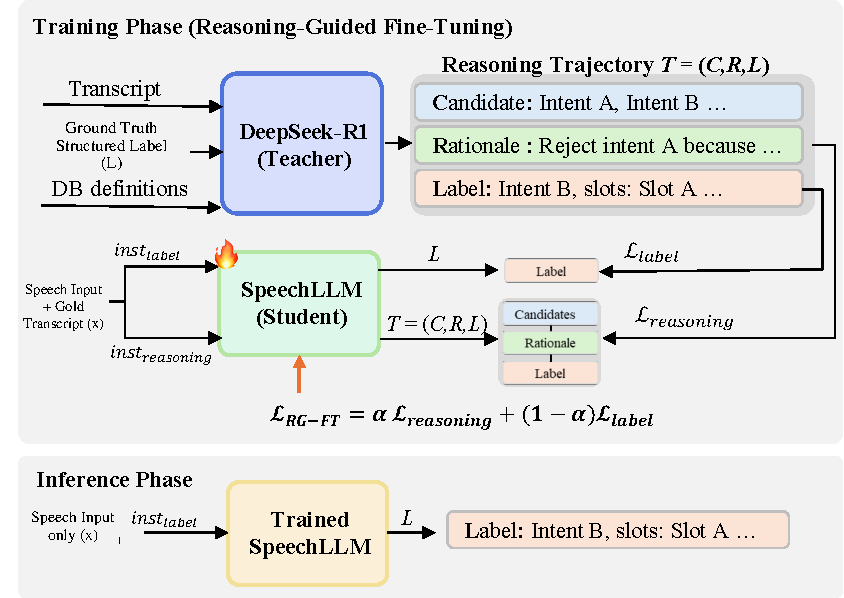
\includegraphics[width=\linewidth]{model_GR_revised.pdf}
  \caption{RG-FTの学習と推論の流れ。学習時には、音声と正解書き起こしをSpeechLLMに入力し、DeepSeek-R1が生成した構造化推論軌跡と正解の構造化ラベルを学習に用いる。推論時には、学習後のSpeechLLMが音声だけから構造化ラベルを直接出力する。図中のLabelは構造化ラベルを表す。}
  \label{fig:proposed_method}
\end{figure}

\subsection{構造化推論軌跡：$T=(C,R,L)$}
本章では、学習時にSpeechLLMに与える発話音声と正解書き起こしの組を入力$x$とする。構造化推論軌跡$T(x)=(C,R,L)$は、入力$x$に含まれる正解書き起こしについて、発話から予測し得る意図とスロット、構造化ラベルに採用しない意図やスロットとその理由、ならびに構造化ラベルを順に記述した出力である。$C$は発話から予測し得る意図とスロットの集合、$R$は構造化ラベルに採用しない意図やスロットとその理由、$L$は構造化ラベルを表す。構造化推論軌跡$T(x)$は、図\ref{fig:prompt}に示すプロンプトを用いて、学習データ作成用の大規模言語モデルDeepSeek-R1~\cite{Guo_2025}に生成させる。

\begin{figure}[htbp]
\centering
\fbox{\begin{minipage}{0.92\linewidth}
\small
\textbf{プロンプト構造}\\[3pt]
\textbf{System:} You are an SLU Logic Analyst. Given [Input] and DB Definitions, output exactly 3 lines (C, R, L). Compare candidates from DB. Cite evidence.\\[2pt]
\textbf{DB Definitions:} \textit{intent and slot definitions}\quad
\textbf{Input:} \textit{transcript, target label}\\
\textbf{C:} List intent candidates; list slot candidates with value candidates.\\
\textbf{R:} For each $c \in C'_I \cup C'_S$, cite evidence why $c$ is incorrect.\\
\textbf{L:} \{\texttt{"Intent"}: \textit{scenario\_action}, \texttt{"entities"}: \textit{[...]}\}
\end{minipage}}
\caption{DeepSeek-R1に構造化推論軌跡を生成させるプロンプトの構成。正解書き起こし、正解の構造化ラベル、および意図とスロットの定義を入力し、候補集合$C$、棄却理由$R$、構造化ラベル$L$を出力させる。}
\label{fig:prompt}
\end{figure}

\paragraph{候補集合（$C$）}
候補集合$C$は、DeepSeek-R1が構造化ラベルを決める前に比較した意図とスロットの集合である。入力$x$に含まれる正解書き起こしと、対象データセットで定義されたすべての意図名、スロット名、およびそれぞれの定義をまとめたデータベース（DB）をDeepSeek-R1に与える。DeepSeek-R1は、$K$個の意図候補と$J$個のスロット候補を列挙する。ここで、意図候補の集合を$C_I$、スロット候補の集合を$C_S$とし、候補集合を次式で定義する。
\begin{equation}
C=(C_I,C_S).
\tag{1}
\end{equation}
また、各スロット$s_j$には、値候補の集合$\{v_{jm}\}_{m=1}^{M_j}$が対応する。
\begin{equation}
C_I=\{c_k\}_{k=1}^{K}, \qquad
C_S=\left\{s_j\left(\{v_{jm}\}_{m=1}^{M_j}\right)\right\}_{j=1}^{J}.
\tag{2}
\end{equation}
ここで、$c_k$は$k$番目の意図候補、$s_j$は$j$番目のスロット種別、$M_j$はスロット$s_j$に対する値候補の数、$v_{jm}$はスロット$s_j$に対する$m$番目の値候補を表す。正解となる意図$y$は、意図候補の集合$C_I$に含める。

\paragraph{棄却理由（$R$）}
棄却理由$R$は、候補集合$C$のうち正解の構造化ラベルに含まれない意図とスロット種別について、それぞれを構造化ラベルに採用しない理由を文章で示した集合である。正解以外の意図候補の集合を$C'_I=C_I\setminus\{y\}$とし、正解の構造化ラベルに含まれないスロット種別候補の集合を$C'_S$とする。各候補$c\in C'_I\cup C'_S$に対し、候補$c$が正解書き起こしの内容に当てはまらない理由$r(c;x)$を生成する。棄却理由$R$は、候補とその理由の組からなる集合として、次式で表される。
\begin{equation}
R=\{(c,r(c;x))\}_{c\in C'_I\cup C'_S}.
\tag{3}
\end{equation}
正解の構造化ラベルに含まれる候補を示すだけでなく、正解以外の各候補を選ばない理由も生成する。これにより、発話中のどの語句が、候補を採用または棄却する根拠となるかをSpeechLLMに学習させる。この設計は、正しい候補と誤った候補を比較し、各候補を選ぶ理由または選ばない理由を示すことで、モデルの判断基準を明確にできるという先行研究の知見に基づく~\cite{chen-etal-2021-kace,shim2024chainofthoughtaugmentationlogitcontrast,verma2021counterfactual}。

\paragraph{構造化ラベル（$L$）}
構造化ラベル$L$は、最終的に予測した意図と、発話から抽出したスロットの種類および値を一つにまとめた結果である。構造化ラベルは、意図$y$と、スロットと値の組$(s_k,v_k)$の集合から構成され、次式で表される。ここで、$s_k$は$k$番目のスロット種別、$v_k$はそれに対応する値を表す。
\begin{equation}
L=\{\mathrm{intent}:y,\ \mathrm{entities}:\{(s_k,v_k)\}_k\}.
\tag{4}
\end{equation}

\subsection{DeepSeek-R1を用いた学習データの構築}
SpeechLLMの学習データを作成するモデルを、本研究では教師モデルと呼ぶ。構造化推論軌跡$T$を含む学習データを作成するため、教師モデルとしてDeepSeek-R1~\cite{Guo_2025}を用いる。DeepSeek-R1には、正解書き起こし、正解の構造化ラベル$(y,S^*)$、ならびに対象データセットで定義されたすべての意図およびスロットの定義を含むデータベースを入力し、構造化推論軌跡$T$を生成させる。ここで、$S^*$は正解となるスロットと値の組の集合を表す。正解の構造化ラベルを入力することで、生成される棄却理由が正解の構造化ラベルと矛盾する危険を抑える。11,514件の発話について生成した出力のうち、94.0\%が所定の$C\rightarrow R\rightarrow L$形式に従っていた。所定の形式で出力されなかった残りの6.0\%は、学習データから除外した。また、DeepSeek-R1が発話ごとに列挙した候補数は、意図候補が平均2.5個、スロット候補が平均1.2個であった。

\subsection{学習方法と目的関数}
構造化推論軌跡と構造化ラベルをどのように学習させるかによる違いを調べるため、3種類の学習方法を比較する。Direct-FTは構造化ラベルだけを学習し、Reasoning-FTは構造化推論軌跡だけを学習する。提案手法のRG-FTは、構造化ラベルと構造化推論軌跡を同時に学習する。

学習では、モデルの出力と正解との差を数値で表した損失を小さくするように、モデル内部の調整値であるパラメータを更新する。構造化推論軌跡$T=(C,R,L)$を含む学習サンプル$(x,T)$に対し、パラメータ$\theta$を持つSpeechLLMの構造化ラベル予測損失と推論軌跡生成損失を、次式で定義する。
\begin{equation}
\ell_{\mathrm{label}}(x)=-\log p_\theta(L\mid x,\mathrm{inst}_{\mathrm{label}}).
\tag{5}
\end{equation}
\begin{equation}
\ell_{\mathrm{reasoning}}(x)=-\log p_\theta(T\mid x,\mathrm{inst}_{\mathrm{reasoning}}).
\tag{6}
\end{equation}
ここで、$p_\theta$は、パラメータ$\theta$を持つSpeechLLMが各出力を生成する確率を表す。$\ell_{\mathrm{label}}(x)$は、入力$x$から構造化ラベル$L$を生成するタスクの損失を表す。$\ell_{\mathrm{reasoning}}(x)$は、候補集合$C$、棄却理由$R$、および構造化ラベル$L$から構成される構造化推論軌跡$T=(C,R,L)$全体を生成するタスクの損失を表す。$\mathrm{inst}_{\mathrm{label}}$と$\mathrm{inst}_{\mathrm{reasoning}}$は、どちらの出力を生成するかをSpeechLLMに伝える指示文である。

\subsubsection{Direct Fine-Tuning（Direct-FT）}
Direct-FTでは、候補集合$C$と棄却理由$R$を生成せず、入力$x$から構造化ラベル$L$を直接予測する。学習方法だけが評価結果に与える影響を比較するため、Choiら~\cite{choi2025exploring}の学習方法を本研究の実験条件下で再実装した。Direct-FTの学習目的関数を次式で定義する。
\begin{equation}
\mathcal{L}_{\mathrm{Direct}}=\frac{1}{|B|}\sum_{x\in B}\ell_{\mathrm{label}}(x).
\tag{7}
\end{equation}
ここで、$B$は、1回のパラメータ更新でまとめて処理する学習サンプルの集合（ミニバッチ）、$|B|$はそのサンプル数を表す。

\subsubsection{Reasoning Fine-Tuning（Reasoning-FT）}
Reasoning-FTでは、構造化推論軌跡$T$全体の生成だけを学習する。構造化ラベル$L$を直接予測するタスクは使用しない。この条件により、構造化推論軌跡だけを学習させた場合の効果を評価する。Reasoning-FTの学習目的関数を次式で定義する。
\begin{equation}
\mathcal{L}_{\mathrm{Reasoning}}=\frac{1}{|B|}\sum_{x\in B}\ell_{\mathrm{reasoning}}(x).
\tag{8}
\end{equation}
推論時には、構造化ラベル$L$を出力する前に、候補集合$C$と棄却理由$R$を生成する。このため、構造化ラベルだけを直接生成する場合よりも推論時間が長くなる。また、候補集合や棄却理由に誤りがあると、その誤りが構造化ラベルの生成にも影響する可能性がある。

\subsubsection{Reasoning-Guided Fine-Tuning（RG-FT、提案手法）}
小規模なモデルに構造化推論軌跡の生成だけを学習させると、構造化ラベルの予測精度が低下する場合があることが報告されている~\cite{li-etal-2025-small-models,chen-etal-2025-unveiling-key,chen-etal-2025-skip}。そこでRG-FTでは、構造化ラベルの予測を主要タスクとし、その学習を支援する補助タスクとして構造化推論軌跡の生成を同時に学習させる~\cite{hsieh-etal-2023-distilling}。構造化ラベルを予測する学習を維持することで、構造化推論軌跡の生成が構造化ラベルの予測を妨げる影響を抑える。また、構造化推論軌跡を生成する学習により、意味の近い意図を選ばない理由も学習させる。RG-FTの目的関数を次式で定義する。
\begin{equation}
\mathcal{L}_{\mathrm{RG\mbox{-}FT}}
=\alpha\frac{1}{|B_G|}\sum_{x\in B_G}\ell_{\mathrm{reasoning}}(x)
+(1-\alpha)\frac{1}{|B_L|}\sum_{x\in B_L}\ell_{\mathrm{label}}(x).
\tag{9}
\end{equation}
ここで、$B_G$は構造化推論軌跡の生成に用いるミニバッチ、$B_L$は構造化ラベルの予測に用いるミニバッチを表す。$\alpha$は二つの損失の重みを決める値であり、値が大きいほど構造化推論軌跡の生成を重視する。推論時には、構造化ラベル予測用の指示文$\mathrm{inst}_{\mathrm{label}}$だけを用いる。このため、RG-FTを適用したSpeechLLMは、候補集合や棄却理由を生成せず、構造化ラベルを直接出力する。

\section{実験条件}
\subsection{データセット}
提案手法の性能を評価するため、SLURP~\cite{bastianelli-etal-2020-slurp}と、Speech-MASSIVE~\cite{lee2024speechmassivemultilingualspeechdataset}のフランス語データ（以下、Speech-MASSIVE（FR））を用いる。SLURPは、カレンダーや電子メールなど18種類の分野と、60種類の意図を収録した英語のデータセットである。学習用に11,514件、開発用に2,033件、テスト用に2,974件の発話を使用する。Speech-MASSIVEは、発話データを収録したMASSIVEコーパスを基に構築された多言語のデータセットである。本研究で使用するSpeech-MASSIVE（FR）が収録する意図の種類と、学習用、開発用、テスト用の発話数はSLURPと同じである。

\subsection{評価指標}
SLURP~\cite{bastianelli-etal-2020-slurp}の評価設定に従い、シナリオ正解率、アクション正解率、意図正解率、およびSLU-F1を用いる。SLURPでは、各発話の意図を、発話の利用分野を表すシナリオと、ユーザーが求める操作を表すアクションの組として定義する。例えば、意図\texttt{calendar\_set}は、カレンダー分野を表すシナリオ\texttt{calendar}と、設定操作を表すアクション\texttt{set}から構成される。本研究では、シナリオとアクションの組合せによって定まる分類上の区分を、意図クラスと呼ぶ。

シナリオ正解率は、シナリオを正しく予測した発話の割合である。アクション正解率は、アクションを正しく予測した発話の割合である。意図正解率は、シナリオとアクションの両方を正しく予測した発話の割合である。SLU-F1は、スロットの種類と値の抽出性能を表す。適合率（Precision）は予測したスロットのうち正しかったものの割合、再現率（Recall）は正解スロットのうち予測できたものの割合を表す。スロットの種類と値の一致度に基づいて両者を求め、その調和平均をSLU-F1とする。

\subsection{潜在空間における分離性の分析}
SpeechLLMは、入力された発話の特徴をベクトルとして内部に保持する。このベクトルが配置される空間を、本研究では潜在空間と呼ぶ。同じ意図クラスの発話から得たベクトルが互いに近く、異なる意図クラスのベクトルが互いに離れているほど、意図クラスの分離性が高いと定義する。

RG-FTによって分離性が向上するかを調べるため、各SpeechLLMが構造化ラベルを生成する際の内部表現を分析する。まず、構造化ラベルを、SpeechLLMが文章を処理する単位（トークン）に分け、シナリオとアクションに対応するトークンを特定する。次に、各トークンの特徴を数値で表した最終層の隠れ状態ベクトルを取得し、その平均を求める。この処理によって発話ごとに得られるベクトルを、意図表現ベクトル$z$と定義する。

意図表現ベクトルの分離性は、Silhouette係数~\cite{ROUSSEEUW198753}、Fisher比~\cite{fisher1936use}、および重心マージンの3種類の指標で評価する。Silhouette係数は、同じ意図クラス内のベクトル間距離と、最も近い別の意図クラスまでの距離を比較する指標である。本研究では、ベクトルの向きの違いを表すコサイン距離と、ベクトル間の直線距離を表すユークリッド距離を用いて、それぞれ算出する。Fisher比は、異なる意図クラス間のばらつきと、同じ意図クラス内のばらつきとの比を表す。Silhouette係数とFisher比は、値が大きいほど意図クラスを分けやすいことを示す。

重心マージンは、各発話のベクトルが、正解クラスの中心にどの程度近く、最も近い別のクラスの中心からどの程度離れているかを表す。ここで、$y$は意図表現ベクトル$z$の正解クラス、$\mu_y$は正解クラス$y$に属する意図表現ベクトルの重心、$d(\cdot,\cdot)$はベクトル間のユークリッド距離を表す。重心マージンを次式で定義する。
\begin{equation}
m(z)=d(z,\mu_{y'})-d(z,\mu_y).
\tag{10}
\end{equation}
$y'$は、正解クラス以外で、意図表現ベクトル$z$に重心が最も近い意図クラスであり、次式で求める。ここで、$\mu_k$は意図クラス$k$の重心を表す。
\begin{equation}
y'=\arg\min_{k\ne y}d(z,\mu_k).
\tag{11}
\end{equation}
したがって、重心マージンは、意図表現ベクトル$z$から最も近い別のクラスの重心までの距離と、正解クラスの重心までの距離との差を表す。値が大きいほど、$z$が、最も近い別のクラスの重心よりも正解クラスの重心に相対的に近いことを示す。

\subsection{評価実験条件}
Choiら~\cite{choi2025exploring}に従い、学習時には発話音声と正解書き起こしの両方を入力として用いる。推論時には、発話音声だけを入力する。実験では、Qwen2.5-Omni-7B~\cite{xu2025qwen25omni}、Qwen2.5-Omni-3B~\cite{xu2025qwen25omni}、Qwen2-Audio-7B~\cite{chu2024qwen2}、Qwen2-Audio-7B-Inst.~\cite{chu2024qwen2}、Audio-Flamingo-3~\cite{goel2025audioflamingo3}、およびMusic-Flamingo~\cite{ghosh2025musicflamingoscalingmusic}の6種類のSpeechLLMを用いる。追加学習条件を表\ref{tab:settings}に示す。

\begin{table}[htbp]
\centering
\caption{SpeechLLMの追加学習条件。}
\label{tab:settings}
\begin{tabular}{ll}
\hline
項目 & 設定値 \\ \hline
パラメータ更新範囲 & 全パラメータ \\
計算精度 & BF16 \\
最適化手法 & AdamW \\
学習率 & $4\times10^{-5}$ \\
学習率スケジュール & コサインアニーリング \\
バッチサイズ & 4 \\
勾配累積ステップ数 & 4 \\
最大エポック数 & 4 \\
新規生成トークンの最大数 & 384 \\
使用GPU & H200 GPU 2台 \\
試行回数 & 3 \\
RG-FTの混合比 & $\alpha=0.5$ \\ \hline
\end{tabular}
\end{table}

学習率は、1回のパラメータ更新で値をどの程度変えるかを決める。バッチサイズは、1回の計算でまとめて処理する学習サンプル数を表す。勾配累積は、複数のミニバッチから得た更新量をまとめてから、パラメータを更新する方法である。新規生成トークンの最大数は、1回の出力長の上限を表す。GPUはSpeechLLMの学習に用いる計算装置である。BF16は、数値を16ビットで表現する浮動小数点形式である。AdamWはパラメータの更新方法、コサインアニーリングは学習の進行に合わせて学習率を変化させる方法を表す。

各SpeechLLMについて、学習データ全体を1回処理する単位（エポック）ごとにモデルの状態をチェックポイントとして保存し、各学習方法の目的関数で定義した損失を開発データ上で算出する。保存したチェックポイントのうち、開発データにおける損失が最も低いものをテストデータの評価に用いる。各実験は、学習データを処理する順序などを決める乱数の初期値（乱数シード）を3種類に変えて実施し、得られた評価値の平均を報告する。

また、学習前に設定する値（ハイパーパラメータ）である$\alpha$が意図正解率とSLU-F1に与える影響を調べる。$\alpha$は、構造化ラベル予測損失と推論軌跡生成損失の重みを調整する。RG-FTでは$\alpha$を0.1から0.9まで0.1刻みで変化させ、評価値の変化を分析する。比較のため、構造化ラベル予測損失だけを用いるDirect-FTを$\alpha=0$、推論軌跡生成損失だけを用いるReasoning-FTを$\alpha=1$として、図\ref{fig:alpha_sensitivity}に併記する。
\begin{equation}
\alpha\in\{0.1,0.2,\ldots,0.9\}.
\tag{12}
\end{equation}

\section{評価結果}
\subsection{RG-FTによるSLU性能の向上}
表\ref{tab:main_results}に、SLURPおよびSpeech-MASSIVE（FR）を用いて、6種類のSpeechLLMに対するDirect-FT、Reasoning-FT、およびRG-FTの評価結果を示す。

\begin{table}[htbp]
\centering
\scriptsize
\setlength{\tabcolsep}{3pt}
\renewcommand{\arraystretch}{1.05}
\caption{SLURPおよびSpeech-MASSIVE（FR）のテストセットにおける主要結果（3種類の乱数シードの平均）。太字はモデル・評価指標ごとの最高値。Sce.: シナリオ正解率、Act.: アクション正解率、Int.: 意図正解率、F1: SLU-F1スコア。}
\label{tab:main_results}
\resizebox{\linewidth}{!}{%
\begin{tabular}{llcccccccccccc}
\hline
 & & \multicolumn{4}{c}{Direct-FT} & \multicolumn{4}{c}{Reasoning-FT ($C \to R \to L$)} & \multicolumn{4}{c}{RG-FT（提案手法）} \\
\cmidrule(lr){3-6}\cmidrule(lr){7-10}\cmidrule(lr){11-14}
データセット & モデル & Sce. & Act. & Int. & F1 & Sce. & Act. & Int. & F1 & Sce. & Act. & Int. & F1 \\
\hline
\multirow{6}{*}{\textit{SLURP}}
 & Qwen2.5-Omni-7B & 91.30 & 88.67 & 87.78 & 76.19 & 89.53 & 86.53 & 85.24 & 74.89 & \textbf{91.81} & \textbf{89.22} & \textbf{88.35} & \textbf{76.88} \\
 & Qwen2.5-Omni-3B & 90.66 & 87.61 & 86.63 & 74.87 & 88.79 & 84.74 & 83.57 & 71.87 & \textbf{91.32} & \textbf{88.55} & \textbf{87.62} & \textbf{75.88} \\
 & Qwen2-Audio-7B & 88.87 & 85.34 & 84.20 & 69.84 & 87.44 & 83.56 & 82.04 & 69.29 & \textbf{90.23} & \textbf{86.64} & \textbf{85.81} & \textbf{72.26} \\
 & Qwen2-Audio-7B-Inst. & 88.97 & 85.36 & 84.26 & 70.09 & 87.14 & 83.39 & 81.73 & 69.87 & \textbf{90.28} & \textbf{87.16} & \textbf{86.31} & \textbf{72.78} \\
 & Audio-Flamingo-3 & 88.30 & 84.51 & 83.23 & 70.22 & 86.83 & 83.05 & 81.51 & 69.44 & \textbf{89.75} & \textbf{86.42} & \textbf{85.25} & \textbf{72.61} \\
 & Music-Flamingo & 87.63 & 84.07 & 82.81 & 69.36 & 86.87 & 82.96 & 81.31 & 69.35 & \textbf{89.81} & \textbf{86.23} & \textbf{85.21} & \textbf{72.16} \\
\hline
\multirow{6}{*}{\shortstack{\textit{Speech-MASSIVE}\\\textit{（FR）}}}
 & Qwen2.5-Omni-7B & 91.60 & 89.16 & 88.05 & 74.62 & 90.33 & 87.08 & 85.98 & 71.90 & \textbf{92.10} & \textbf{89.82} & \textbf{88.71} & \textbf{75.68} \\
 & Qwen2.5-Omni-3B & 91.06 & 88.44 & 87.11 & 73.22 & 88.76 & 85.66 & 84.32 & 70.21 & \textbf{91.22} & \textbf{88.79} & \textbf{87.68} & \textbf{74.22} \\
 & Qwen2-Audio-7B & 89.26 & 85.88 & 84.52 & 67.78 & 88.20 & 84.59 & 82.99 & 67.38 & \textbf{90.29} & \textbf{87.90} & \textbf{86.62} & \textbf{69.96} \\
 & Qwen2-Audio-7B-Inst. & 89.09 & 85.83 & 84.43 & 68.15 & 87.93 & 84.23 & 82.78 & 66.79 & \textbf{90.32} & \textbf{88.13} & \textbf{86.79} & \textbf{70.59} \\
 & Audio-Flamingo-3 & 88.64 & 85.64 & 84.13 & 68.02 & 87.73 & 84.72 & 83.02 & 65.96 & \textbf{90.96} & \textbf{87.83} & \textbf{86.67} & \textbf{70.80} \\
 & Music-Flamingo & 89.07 & 86.03 & 84.62 & 69.48 & 87.73 & 84.08 & 82.77 & 67.42 & \textbf{90.43} & \textbf{87.97} & \textbf{86.70} & \textbf{71.18} \\
\hline
\end{tabular}%
}
\end{table}

RG-FTは、すべてのモデル、評価指標、およびデータセットの組合せにおいて、Direct-FTとReasoning-FTを上回った。また、表\ref{tab:main_results}では、Direct-FTの意図正解率とSLU-F1が低いモデルほど、RG-FTによる両評価指標の向上幅が大きい傾向が見られた。SLURPのMusic-Flamingoでは、Direct-FTと比べて、意図正解率が2.40ポイント、SLU-F1が2.80ポイント向上した。Direct-FTの意図正解率とSLU-F1が最も高いQwen2.5-Omni-7Bでも、両評価指標が向上した。

一方、Reasoning-FTは、モデル、評価指標、およびデータセットのすべての組合せでDirect-FTを下回った。SLURPのQwen2.5-Omni-3Bでは、Direct-FTと比べて意図正解率が3.06ポイント低下した。Reasoning-FTでは、候補集合、棄却理由、構造化ラベルからなる長い出力を順に生成する必要がある。この出力の生成がモデルの負担となり、構造化ラベルの予測を妨げた可能性がある。特に、規模の小さいモデルほど性能低下が大きい傾向は、小規模なモデルに構造化推論軌跡だけを学習させることの難しさを報告した先行研究~\cite{li-etal-2025-small-models,chen-etal-2025-unveiling-key,chen-etal-2025-skip}と一致する。

RG-FTは、構造化ラベルを直接予測する学習を維持しながら、構造化推論軌跡の生成も同時に学習する。この学習方法により、構造化ラベルの予測を妨げる影響を抑えながら、意味の近い意図を選ばない理由を学習に取り入れられたと考えられる。以上より、構造化推論軌跡の生成は、構造化ラベルの予測に置き換えて単独で学習させるのではなく、構造化ラベルの予測と組み合わせることが、意図正解率とSLU-F1の向上に有効である。特に、Direct-FTの意図正解率とSLU-F1が低いSpeechLLMで大きな改善が得られた。

\subsection{RG-FTによる意図クラスの分離性向上}
表\ref{tab:rep_analysis}に、Qwen2.5-Omni-7BとQwen2.5-Omni-3Bについて、Direct-FTとRG-FTの潜在空間における意図クラスの分離性を示す。RG-FTは、両モデルで、表に示す4つの評価値をすべて改善した。

\begin{table}[htbp]
\centering
\small
\caption{Direct-FTとRG-FTの潜在空間における意図クラスの分離性。すべての指標は、値が高いほど意図クラスを分けやすいことを示す。}
\label{tab:rep_analysis}
\resizebox{\linewidth}{!}{%
\begin{tabular}{lcccc}
\hline
 & \multicolumn{2}{c}{\textbf{Qwen2.5-Omni-7B}} & \multicolumn{2}{c}{\textbf{Qwen2.5-Omni-3B}} \\
\cmidrule(lr){2-3}\cmidrule(lr){4-5}
\textbf{指標} & \textbf{Direct-FT} & \textbf{RG-FT} & \textbf{Direct-FT} & \textbf{RG-FT} \\ \hline
 Silhouette係数（コサイン距離） & 0.242 & \textbf{0.279} & 0.299 & \textbf{0.332} \\
 Silhouette係数（ユークリッド距離） & 0.157 & \textbf{0.176} & 0.195 & \textbf{0.219} \\
Fisher比 & 1.133 & \textbf{1.276} & 1.521 & \textbf{1.839} \\
重心マージン & 0.174 & \textbf{0.194} & 0.208 & \textbf{0.230} \\ \hline
\end{tabular}%
}
\end{table}

Qwen2.5-Omni-7Bでは、コサイン距離に基づくSilhouette係数が、Direct-FTの0.242からRG-FTの0.279へ0.037ポイント向上した。Qwen2.5-Omni-3Bでは、Fisher比が、Direct-FTの1.521からRG-FTの1.839へ0.318ポイント向上した。また、コサイン距離とユークリッド距離のどちらを用いた場合もSilhouette係数が向上したため、改善は特定の距離の測り方だけに依存していない。

これらの結果は、Direct-FTと比べて、RG-FTでは同じ意図クラスの意図表現ベクトルが近くに集まり、異なる意図クラスのベクトルが離れて配置されたことを示す。したがって、構造化推論軌跡を学習に取り入れることで、SpeechLLMの内部に意図クラスを分けやすい表現が形成されたと考えられる。

分離性指標の改善は、表\ref{tab:main_results}に示した意図正解率の向上とも整合する。RG-FTによる意図クラスの分離性向上が、意味の近い意図の取り違えを減らし、意図正解率の向上に寄与した可能性がある。

\subsection{構造化推論軌跡の各要素の効果}
表\ref{tab:ablation_components}に、構造化推論軌跡を構成する要素を段階的に追加した場合の評価結果を示す。本実験では、SLURPで学習したQwen2.5-Omni-3Bを評価した。

\begin{table}[htbp]
\centering
\small
\caption{構造化推論軌跡の各要素が評価値に与える影響（SLURPで学習したQwen2.5-Omni-3B）。RG-FTの各条件では、表に示す要素の生成と構造化ラベルの直接予測を同時に学習する。}
\label{tab:ablation_components}
\resizebox{\linewidth}{!}{%
\begin{tabular}{lcc}
\hline
\textbf{設定（学習する出力）} & \textbf{Sce. / Act. / Int.} & \textbf{SLU-F1} \\ \hline
Direct-FT（補助出力なし） & 90.66 / 87.61 / 86.63 & 74.87 \\
RG-FT（構造化ラベル + $C$） & 90.95 / 87.96 / 87.03 & 75.57 \\
RG-FT（構造化ラベル + $C \to R$） & 91.20 / 88.44 / 87.57 & 75.62 \\
\textbf{RG-FT（構造化ラベル + $C \to R \to L$）} & \textbf{91.32 / 88.55 / 87.62} & \textbf{75.88} \\ \hline
\end{tabular}%
}
\end{table}

構造化ラベルの直接予測に候補集合$C$の生成を加えた条件では、意図正解率がDirect-FTの86.63から87.03へ、SLU-F1が74.87から75.57へ向上した。正解と混同しやすい意図も学習時に列挙することで、SpeechLLMが比較すべき意図を捉えやすくなった可能性がある。

候補集合$C$に棄却理由$R$を加えた条件では、意図正解率が87.03から87.57へ向上した。候補を列挙するだけでなく、正解以外の候補を選ばない理由も学習させることで、発話が表す意図と、意味の近い意図との違いを捉えやすくなった可能性がある。

さらに、構造化ラベル$L$まで含む$C\rightarrow R\rightarrow L$を用いた条件では、シナリオ正解率、アクション正解率、意図正解率、およびSLU-F1のすべてにおいて最も高い値が得られた。意図正解率はDirect-FTの86.63から87.62へ、SLU-F1は74.87から75.88へ向上した。

以上より、候補集合$C$は比較対象となる意図を示し、棄却理由$R$は正解以外の意図を選ばない理由を示し、構造化ラベル$L$は比較と棄却を経て選んだ意図とスロットを示す。これらを順に追加することで、Qwen2.5-Omni-3Bの評価値は段階的に向上した。

\subsection{構造化ラベル予測損失と推論軌跡生成損失の混合比$\alpha$の感度分析}
\begin{figure}[htbp]
  \centering
  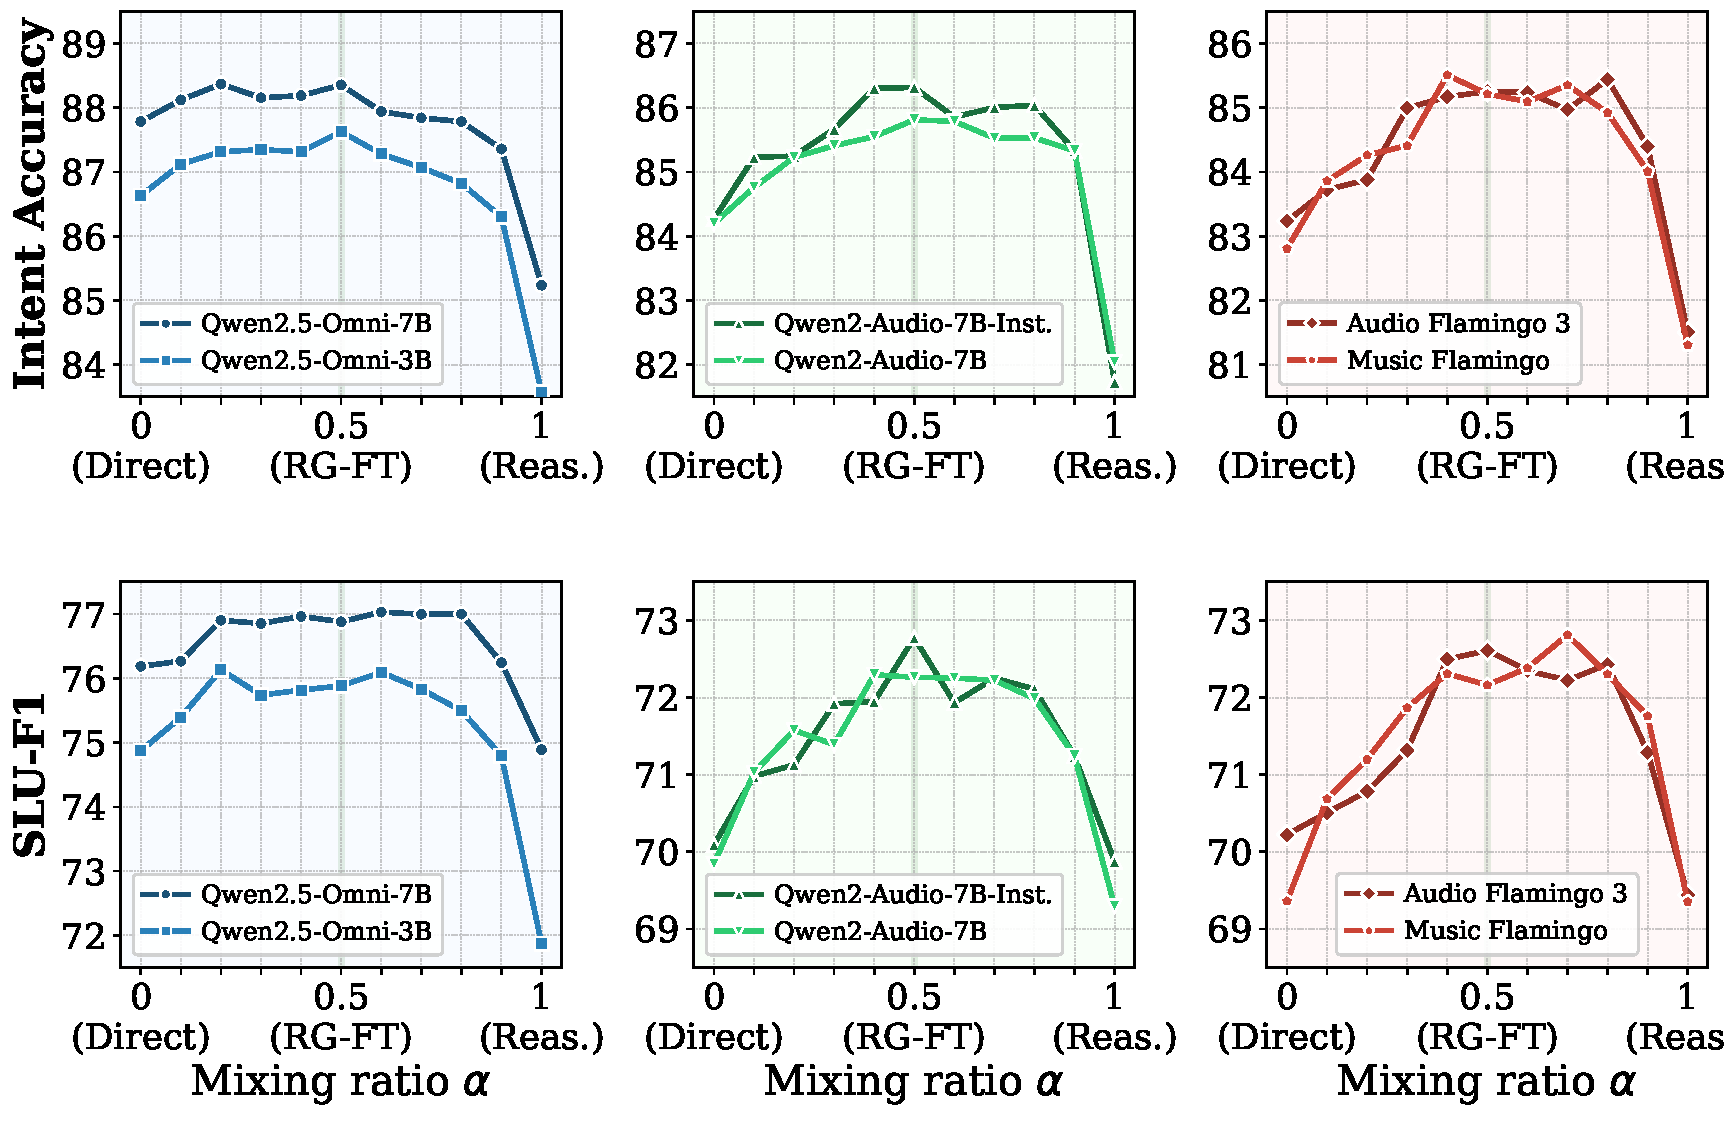
\includegraphics[width=\linewidth]{sensitivity_of_a.pdf}
  \caption{6種類のSpeechLLMにおける混合比$\alpha$と、SLURPテストデータでの意図正解率（上段）およびSLU-F1（下段）との関係。$\alpha=0$はDirect-FT、$\alpha=1$はReasoning-FTに対応し、$\alpha=0.5$は主実験で用いたRG-FTの設定である。各値は3種類の乱数シードによる評価の平均。}
  \label{fig:alpha_sensitivity}
\end{figure}

図\ref{fig:alpha_sensitivity}に、SLURPで学習した6種類のSpeechLLMについて、混合比$\alpha$を変化させた場合の意図正解率とSLU-F1を示す。混合比$\alpha$は、構造化ラベル予測損失と推論軌跡生成損失のどちらを重く扱うかを決める。$\alpha=0$は構造化ラベル予測損失だけを用いるDirect-FT、$\alpha=1$は推論軌跡生成損失だけを用いるReasoning-FTに対応する。$0<\alpha<1$では、二つの損失を組み合わせる。

すべてのSpeechLLMで、$0<\alpha<1$の範囲に、$\alpha=0$および$\alpha=1$よりも意図正解率とSLU-F1が高い設定があった。この結果は、構造化ラベルの予測と構造化推論軌跡の生成のどちらか一方だけでなく、両方を組み合わせて学習させることで、二つの評価指標を向上できることを示す。

ただし、意図正解率またはSLU-F1が最も高くなる$\alpha$を超えて推論軌跡生成損失を重くすると、両評価指標は低下する傾向を示した。構造化推論軌跡の生成を重視しすぎると、構造化ラベルの予測が妨げられる可能性がある。この傾向は、4.1節でReasoning-FTがDirect-FTを下回った結果と一致する。

Direct-FTの意図正解率とSLU-F1が比較的高いQwen2.5-Omniでは、$\alpha$を変化させた場合の両評価指標の変化幅が比較的小さかった。一方、Direct-FTの両評価指標が比較的低いSpeechLLMでは、$0<\alpha<1$とすることによる性能向上が大きかった。また、Direct-FTの両評価指標が比較的低いSpeechLLMでは、各評価指標が最も高くなる$\alpha$は、主に$\alpha\in[0.4,0.6]$の範囲に位置した。

以上の傾向から、Direct-FTの意図正解率とSLU-F1が低いモデルほど、構造化推論軌跡を追加して学習させる効果が大きい可能性がある。いずれのSpeechLLMでも、二つの損失を同じ重みで用いる$\alpha=0.5$では、意図正解率とSLU-F1が各モデルの最高値またはその近傍となった。したがって、本実験の範囲では、モデルごとに$\alpha$を調整しない場合でも、$\alpha=0.5$を用いることで、Direct-FTおよびReasoning-FTより高い性能を得られる可能性がある。

\section{失敗及びあい路事項}
本研究の実施において、報告すべき失敗およびあい路事項はなかった。

\section{安全性の検討}
本研究は、音声言語理解のアルゴリズムを評価するものであり、機器の制御や人の身体に関わる作業は対象としていない。このため、実験の実施に伴う直接的な安全上の問題はない。ただし、提案手法を実際の対話システムに組み込む場合、意図やスロットの誤予測によって、ユーザーの要求と異なる処理が実行される可能性がある。実用化に当たっては、誤予測時に処理を停止する仕組みや、処理の実行前にユーザーへ確認する仕組みを、用途に応じて設ける必要がある。

\section{環境影響に関する検討}
SpeechLLMの学習にはH200 GPUを2台使用しており、計算に伴って電力を消費する。一方、本研究では消費電力量を測定していないため、環境負荷の大きさは定量的に評価していない。

\section{本研究の水準比較}
本研究の位置付けを示すため、日本電気株式会社（NEC）が提供するコンタクトセンター向けAIソリューション「NEC Communication Agent」との比較を表\ref{tab:comparison}に示す。NEC Communication Agentは製品であるのに対し、本研究の対象はSpeechLLMの学習方法である。このため、製品全体の性能ではなく、推論時に入力音声を言語処理する構成を比較する。

公開情報によると、NEC Communication Agentは、電話対応にNEC独自の音声認識エンジンを用いて発話を文字起こしし、大規模言語モデル（LLM）と対話制御機能を用いて問い合わせへの回答を生成する~\cite{nec_communication_agent}。すなわち、音声認識と後段の言語処理を分けた構成である。この構成では、音声認識の誤りが後段の回答生成に影響する可能性がある。一方、本研究では、学習時には音声と正解書き起こしをSpeechLLMに入力するが、推論時には音声だけを入力する。したがって、推論時には独立した音声認識結果を経由せず、一つのSpeechLLMが音声から構造化ラベルを直接予測する。さらに、声の抑揚、話す速さ、声質などの音声情報は、推論時に入力する音声の一部としてSpeechLLMに与えられる。ただし、本研究では、これらの音声情報が意図分類に与える影響を個別には評価していない。また、両者の処理時間や性能を同じ条件で測定していないため、表\ref{tab:comparison}は推論時の入力と処理構成の違いだけを示す。

\begin{table}[htbp]
\centering
\caption{本研究とNEC Communication Agent~\cite{nec_communication_agent}における推論時の入力および処理構成の違い。処理時間や性能の実測比較ではない。}
\label{tab:comparison}
\begin{tabularx}{\linewidth}{>{\raggedright\arraybackslash}p{38mm}XX}
\hline
比較項目 & 本研究 & NEC Communication Agent~\cite{nec_communication_agent} \\ \hline
推論時に言語処理へ与える入力 & 音声 & 音声認識結果のテキスト \\
処理構成 & 一つのSpeechLLMが音声を直接処理 & 音声認識、LLM、および対話制御を組み合わせて処理 \\
音声に含まれる情報の入力 & 音声の一部としてSpeechLLMに入力 & 後段の言語処理に与えるテキストには含まれない \\
独立した音声認識の使用 & 使用しない & 使用する \\ \hline
\end{tabularx}
\end{table}

\section{知的所有権の状況及び検討}
本研究に関連する知的所有権として、音声データを用いた作業支援に関する自社特許と、対話システムにおける意図分類に関する他社特許を調査した。調査した特許の概要を以下に示す。

\subsection{自社特許の状況}
\paragraph{No. 1}
\begin{tabularx}{\linewidth}{>{\raggedright\arraybackslash}p{35mm}X}
\hline
項目 & 内容 \\ \hline
出願依頼受付番号 & 342100752 \\
出願番号 & P2022-004540 \\
公開番号 & P2023-103803 \\
公報番号 & 特願 2022-4540 \\
出願年月日 & 2022/01/14 \\
発明者 & 高橋 貴史、小窪 浩明、山本 正明、中西 貴洋 \\
発明の名称 & キーワード辞書作成方法、作業支援方法、キーワード辞書作成システム及び作業支援システム \\
内容の要点 & 作業支援システムで活用するキーワード文字列を、従業員の音声データから自動的に抽出する \\
研究の種類 & （HGNE）依頼研究 \\ \hline
\end{tabularx}

\subsection{他社特許の状況}
\paragraph{No. 1}
\begin{tabularx}{\linewidth}{>{\raggedright\arraybackslash}p{35mm}X}
\hline
項目 & 内容 \\ \hline
出願人 & ジェネシス クラウド サービシーズ インコーポレイテッド \\
公開番号 & 特開2025-118917 \\
公報番号 & - \\
出願年月日 & 2025/05/16 \\
発明の名称 & コンタクトセンターシステムとそのユーザとの間の対話を管理するためのシステム及び方法 \\
内容の要点 & 対話中のユーザ意図を検出し、コンテキスト切替えや行動ツリーを用いて応答処理を動的に変更することで、コンタクトセンターにおける自動的な対話管理を実現する \\ \hline
\end{tabularx}

\paragraph{No. 2}
\begin{tabularx}{\linewidth}{>{\raggedright\arraybackslash}p{35mm}X}
\hline
項目 & 内容 \\ \hline
出願人 & アリババ・グループ・ホールディング・リミテッド \\
公開番号 & 特表2020-537777 \\
公報番号 & - \\
出願年月日 & 2018/10/16 \\
発明の名称 & 発言のユーザ意図を識別するための方法および装置 \\
内容の要点 & 会話履歴から取得した関連発言の情報を利用し、対象発言のユーザ意図を高精度に推定する \\ \hline
\end{tabularx}

\section{結言}
\subsection{結論}
本研究では、意図分類で扱う意図に意味の近いものが複数ある場合に、意味の近い意図を取り違えにくくすることを目的として、Reasoning-Guided Fine-Tuning（RG-FT）を提案した。本研究は先行研究の入力条件を踏襲し、学習時には音声と正解書き起こしをSpeechLLMに入力し、推論時には音声だけを入力する。従来法は、構造化ラベルだけを追加学習の出力に用いる。これに対し、RG-FTは、発話が表す意図と、それに意味の近い意図との違いを説明する構造化推論軌跡も追加学習に用いる。本研究で得られた成果を以下に示す。

\begin{enumerate}
\item \textbf{構造化推論軌跡を用いたSpeechLLMの学習方法}

DeepSeek-R1を用いて、候補集合、正解以外の候補を選ばない理由、および構造化ラベルからなる構造化推論軌跡を生成した。RG-FTでは、構造化ラベルの直接予測と構造化推論軌跡の生成をSpeechLLMに同時に学習させる。この同時学習により、発話が表す意図だけでなく、意味の近い意図を選ばない理由も学習に用いる。

\item \textbf{複数のSpeechLLMにおける音声言語理解性能の向上}

SLURPとSpeech-MASSIVE（FR）の二つのデータセットを用いて、6種類のSpeechLLMにRG-FTを適用した。RG-FTは、モデル、評価指標、およびデータセットのすべての組合せで、構造化ラベルだけを学習するDirect-FTを上回った。SLURPのMusic-Flamingoでは、意図正解率が82.81\%から85.21\%へ2.40ポイント向上し、SLU-F1が69.36から72.16へ2.80ポイント向上した。Direct-FTの意図正解率とSLU-F1が最も高いQwen2.5-Omni-7Bでも、両評価指標が向上した。以上より、本実験で用いた6種類のSpeechLLMと英語・フランス語のデータでは、RG-FTによる一貫した性能向上を確認した。

\item \textbf{潜在空間における意図クラスの分離性向上}

学習後のSpeechLLMから意図表現ベクトルを抽出し、Silhouette係数、Fisher比、および重心マージンを用いて、潜在空間における意図クラスの分離性を分析した。Qwen2.5-Omni-7Bでは、RG-FTの適用により、コサイン距離に基づくSilhouette係数が0.242から0.279へ、Fisher比が1.133から1.276へ、重心マージンが0.174から0.194へ向上した。Qwen2.5-Omni-3Bでも、すべての分離性指標が改善した。分離性指標の改善は、構造化推論軌跡を追加学習に用いることで、同じ意図クラスの内部表現が近くに集まり、異なる意図クラスの内部表現が離れたことを示す。
\end{enumerate}

以上より、本実験の条件では、RG-FTは、推論時には音声だけを入力し、構造化推論軌跡を生成することなく、意味の近い意図に対するSpeechLLMの意図分類性能を向上させた。

\subsection{今後の課題}
本研究では、DeepSeek-R1が生成した構造化推論軌跡を使用したが、構造化推論軌跡に含まれる説明文の正確さや詳しさがSpeechLLMの性能に与える影響は分析していない。今後は、教師モデルを変更した場合に、生成される構造化推論軌跡の品質とSpeechLLMの意図分類性能がどのように変化するかを調べる。また、本研究の教師モデルは正解書き起こしを入力とするため、声の抑揚、話す速さ、感情表現、背景雑音などの音声情報を構造化推論軌跡の生成に利用していない。今後は、教師モデルに音声も入力して構造化推論軌跡を生成する方法と、その方法が意図分類性能に与える影響を検証する。さらに、異なる利用分野や言語のデータでRG-FTを評価し、提案手法を適用できる範囲を調べる。

\clearpage
\section{参考文献}
\begingroup
\renewcommand{\section}[2]{}
\bibliographystyle{unsrt}
\bibliography{mybib,references_additional}
\endgroup

% DUMMY文献は introduction/references_additional.bib 内で「DUMMY」を検索して差し替えること。
% 第12章および第13章の本文は未提供のため未収録。

\end{document}
